\documentclass{article}
\usepackage{graphicx} % inserting images
\usepackage{listings} % for code snippet
\usepackage{mdframed} 
\title{Practical Work 1: TCP File Transfer}
\author{Cuong Pham Khuong BI12-070}

\date{March 2024}

\begin{document}

\maketitle 

\section{Protocol Design}
here is the protocol design
\begin{figure}[h!]
    \centering
    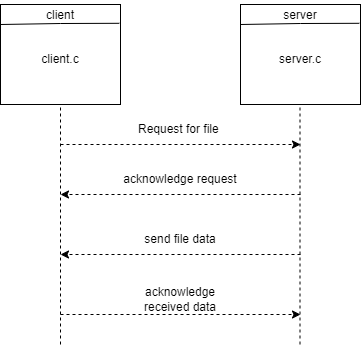
\includegraphics[width=0.5\linewidth]{protocol_design.drawio (1).png}
    \caption{\textit{protocol design}}
    \label{fig:enter-label}
\end{figure}
\subparagraph{The protocol includes the following steps:}
\begin{enumerate}
    \item Client Request: The client initiates the file transfer by sending a request to the server.
    \item Server Response: The server acknowledges the request and prepares to send the file.
    \item File Transfer: The server sends the file to the client.
    \item Completion Acknowledgment: The client acknowledges the successful receipt of the file.
\end{enumerate}
\section{System Organization}
here is the system organization 
\begin{figure}[h!]
    \centering
    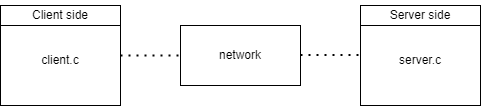
\includegraphics[width=0.5\linewidth]{system organize.drawio.png}
    \caption{\textit{system organization}}
    \label{fig:enter-label}
\end{figure}
\section{File Transfer Implementation}
The \texttt{server.c} file, the function \texttt{send\_file()} is responsible for sending the contents of a file to the client. It opens the file in read-only mode and reads its contents into a buffer. Then, it writes the buffer to the socket and sends the file content to the client.
\begin{mdframed}
    \begin{lstlisting}
    void send_file(int sockfd, char *filename) {
    char buff[MAX];
    int fd = open(filename, O_RDONLY);
    if (fd < 0) {
        printf("Error opening file.\n");
        return;
    }

    while (1) {
        int bytes_read = read(fd, buff, MAX);
        if (bytes_read <= 0) break;
        write(sockfd, buff, bytes_read);
    }
    close(fd);
}
    \end{lstlisting}
\end{mdframed}

In the \texttt{client.c} file, the function \texttt{receive\_file()} is responsible for receiving the file contents sent by the server. It opens (or creates if it doesn't exist) a file named \texttt{client\_file.txt} in write-only mode and reads data from the socket into a buffer. Then, it writes the buffer to the file until there is no more data to read.


\begin{mdframed}
    \begin{lstlisting}
        void receive_file(int sockfd, char *filename) {
    char buff[MAX];
    int fd = open(filename, O_WRONLY | O_CREAT | 
    O_TRUNC, 0666);
    if (fd < 0) {
        printf("Error creating/opening file.\n");
        return;
    }

    while (1) {
        int bytes_read = read(sockfd, buff, MAX);
        if (bytes_read <= 0) break;
        write(fd, buff, bytes_read);
    }
    close(fd);
}
    \end{lstlisting}
\end{mdframed}

\section{Responsibilities}
\subparagraph{In the system:}
\begin{itemize}
    \item The client initiates the file transfer request.
    \item The server listens for incoming requests and handles them accordingly.
    \item Both client and server communicate over the network using TCP sockets.
\end{itemize}
\end{document}
